\section{Architettura}

L'architettura del sistema è stata definita attraverso il deployment diagram mostrato in figura \ref{fig:DeployementFreeStyle}, espresso in notazione free style.
Anzitutto si identifica un pattern architetturale multi-layer, dove:
\begin{enumerate}
\item Il Presentation Layer è costituito dalle applicazioni lato client che vengono utilizzate dagli utenti e hanno il solo compito di recuperare le informazioni dal sistema e visualizzarle, oltre che permettere all'utente d'interagire con il servizio;
\item L'Application Layer gestisce la logica di business. È costituito da tre macro-sistemi specializzati:
\begin{itemize}
    \item \textbf{Gestore profilo}, responsabile di tutto ciò che riguarda i profili degli utenti, come gestire la registrazione, il login
    e soddisfare le query inerenti all'utente. Questo gestore si connette ai servizi di Firebase per gestire l'autenticazione in fase di login;
    \item \textbf{Gestore escursione}, responsabile di gestire le richieste inerenti alle escursioni, come ottenere una lista o i dettagli di uno specifico
    evento. Per fornire informazioni meteorologiche riguardo agli eventi, il gestore si connette ai servizi di Visual Crossing tramite API call. La risposta viene elaborata
    in loco e restituita al client in un formato più breve da definirsi in futuro;
    \item \textbf{Gestore prenotazioni}, responsabile di gestire le richieste riguardanti le prenotazioni che gli utente possono far per ogni evento.
\end{itemize}
\item Il Data Layer si occupa della persistenza dei dati ed è costituito da un database relazionale dove sono conservate le informazioni di ogni evento e utente registrato alla piattaforma.
\end{enumerate}
Inoltre identifichiamo pattern client-server dove il client è costituito dalla mobile app e si interfaccia con il server attraverso l'API gateway.

\begin{figure}[ht!]
    \centering
    \begin{subfigure}{0.9\textwidth}
        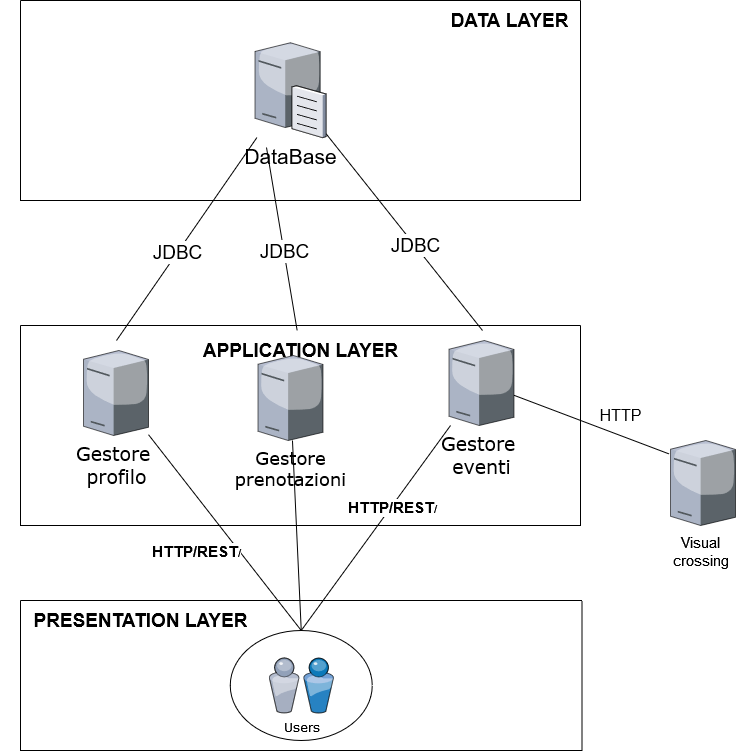
\includegraphics[width=\linewidth]{Iterazione 0/immagini/DeployementFreeStyle(1).png}
    \end{subfigure}
    \caption{Deployment Diagram in versione free style}
    \label{fig:DeployementFreeStyle}
\end{figure}
